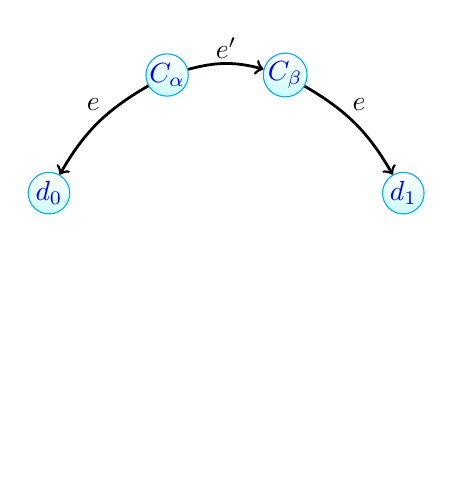
\begin{tikzpicture}[scale=0.75]


\tikzset{label/.style={minimum size=15pt,inner sep=0pt,},}
\tikzset{conf/.style={circle,minimum size=15pt,inner sep=0pt,draw, top color=white ,bottom color=cyan!20, cyan,text=blue},}

\tikzset{camminoUp/.style={->, line width=1pt, snake=coil, segment amplitude=1pt, segment aspect=0, segment length=4mm}}
\tikzset{camminoDown/.style={->, line width=1pt, snake=coil, mirror snake, segment amplitude=1pt, segment aspect=0, segment length=4mm}}



	\draw
		(6,4) node[conf] (d0) {$d_0$}
		(8,6) node[conf] (c0) {$C_\alpha$}
		(10,6) node[conf] (c1) {$C_\beta$}
		(12,0) node[label] (e1) {}
		(12,4) node[conf] (d1) {$d_1$};
		
	\draw[->,line width=1pt](c0) to [bend right=15] (d0);\draw(6.75,5.5)node[label]{$e$};

	\draw[->,line width=1pt](c0) to [bend left=15] (c1);\draw(9,6.45)node[label]{$e'$};
	\draw[->,line width=1pt](c1) to [bend left=15] (d1);\draw(11.25,5.5)node[label]{$e$};

	
\end{tikzpicture}